\documentclass[14pt]{article}
\usepackage{graphicx}
\graphicspath{ {./img/} }
\usepackage{wrapfig}
\usepackage[utf8]{inputenc}
\usepackage[russian]{babel}
\usepackage{amsmath,amsfonts,amssymb,amsthm,epsfig,epstopdf,titling,url,array}

\title{Математические модели в естествознании}
\author{Кочкарев Алексей, 401}
\date{Май 2020}

\newtheorem{definition}{Определение}
\newtheorem{theorem}{Теорема}

\begin{document}

\maketitle

\section*{Аннотация}
Данная работа представляет собой краткий конспект лекций, прочитанных Тихоновым Иваном Владимировичом на факультете ВМК МГУ весной 2020 года перед самым началом пандемии. \\ Во второй главе находятся интересные факты про ударные волны и условие Гюгонио.
\newlineТемы: 
интегральная форма записи для квазилинейного уравнения \\ $u_{t}+(f(u))_{x}=0$,
понятие обобщенного и разрывного обобщенного решения, соотношения Гюгонио, формула скорости движения разрыва для уравнения Хопфа, примеры простейших разрывных решений для уравнения Хопфа, решения со слабыми
разрывами и уравнение линии слабого разрыва.

\section{Конспект лекций}
Рассмотрим уравнение вида: 
\begin{equation}\label{eq:qlinear}
    u_{t}+(f(u))_{x}=0, \ u=u(x,t) - ?
\end{equation}
Зафиксируем отрезок $a\leq x \leq b$ и проинтегрируем по нему уравнение:
$$\int_{a}^{b} u_{t} dx + \int_{a}^{b}(f(u))_{x} dx = 0$$
$$ \frac{d}{dt} \int_{a}^{b} u(x,t)dx + f(u(b,t)) - f(u(a,t))=0 $$
Получаем интегральную форму записи уравнения (\ref{eq:qlinear}):
\begin{equation}\label{eq:int_qlinear}
    \frac{d}{dt} \int_{a}^{b} u(x,t)dx = f(u(a,t))-f(u(b,t))
\end{equation}

\theoremstyle{definition}
\begin{definition}
    Функция $u=u(x,t)$ называется \textbf{обобщенным решением} уравнения (\ref{eq:qlinear}), если она удовлетворяет (\ref{eq:int_qlinear}) при $\forall$ выборе отрезка $[a,b]$ и $\forall t > 0$.
\end{definition}

 \noindent Рассмотрим следующую ситуацию:
\newline
\newline
\begin{equation}\label{eq:u_cases}
    u(x,t) = 
    \begin{cases}
        u_{1}(x, t) & x < \psi(t) ,\\
        u_{2}(x,t) & x > \psi(t)
    \end{cases}
\end{equation}
Здесь $u_{1}(x,t), \ u_{2}(x,t)$ - классические решения уравнения (\ref{eq:qlinear}) в соответствующих областях, $x = \psi (t)$ - линия сильного разрыва с ненулевым скачком функции $[u(t)] = u_{2}(\psi (t),t) - u_{1}(\psi (t), t) \neq 0 \ \forall t \in [0, T]$.
\newline
При каком условии такая функция является обобщенным решением уравнения (\ref{eq:qlinear}) в полосе $(x,\;t) \in (-\infty,\;+\infty) \times [0,\;T]$?
\\Выберем отрезок $[a, b]: \ a < \psi (t) < b, \ 0 \leq t \leq T.$
\\ Распишем тождество (\ref{eq:int_qlinear}):
$$
    \frac{d}{dt}\int_{a}^{b} u(x,t)dx = \frac{d}{dt} \int_{a}^{\psi (t)} u_{1}(x,t) dx + \frac{d}{dt} \int_{\psi(t)}^{b} u_{2}(x, t) dx
$$
По формуле Лейбница имеем:
$$
    u_{1}(\psi(t),t)\psi'(t) + \int_{a}^{\psi(t)} u_{1_{t}}(x,t)dx - 
    u_{2}(\psi(t),t)\psi'(t) + \int_{\psi(t)}^{b} u_{2_{t}}(x,t)dx =
$$
$$
     = (u_{1}(\psi(t),t) - u_{2}(\psi(t),t))\psi'(t)
     + \int_{a}^{\psi(t)} (-(f(u_1)))_{x} dx
     + \int{\psi(t)}^{b} (-(f(u_2)))_{x} dx =
$$
$$
    = -[u(t)]\psi'(t)- (f(u_{1}(\psi(t),t)) - f(u_{1}(a,t))) - 
    - (f(u_{2}(b,t)) - f(u_{2}(\psi(t),t))) = 
$$
$$
    = -[u(t)]\psi'(t) + f(u_{2}(\psi(t), t)) - f(u_1(\psi(t),t)) + 
    f(u_{1}(a,t))-f(u_{2}(b,t))=
$$
$$
        = [f(u)](t) - [u](t)\psi'(t) + f(u(a,t)) - f(u(b,t))\stackrel{(\ref{eq:int_qlinear})}{=}
        f(u(a,t)) - f(u(b,t))
$$
Для выполнения уравнения (\ref{eq:int_qlinear}) необходимо и лостаточно выполнение условия:
$$
    [f(u)](t) - [u](t)\psi'(t) = 0 \ \forall t \in [0, \ T]
$$
Причем $[u](t) \neq 0 \ t \in [0, \; T]$ из-за сильного разрыва.
\newline
\newline
Получаем \textbf{условие Гюгонио}:
\begin{equation}\label{eq:gugonio}
    \psi'(t) = \frac{[f(u)](t)}{[u](t)} = \frac{f(u_2) - f(u_1)}{u_2-u_1}=
    \frac{f(u_{2}(\psi(t),t)) - f(u_{1}(\psi(t), t))}{u_{2}(\psi(t),t)-u_{1}(\psi(t), t)},
    \; 0<t<T
\end{equation}

\theoremstyle{theorem}
\begin{theorem}
Функция $u(x,t)$ вида (\ref{eq:u_cases}) является обобщенным решением уравнения (\ref{eq:qlinear}) \Leftrightarrow \text{всюду на разрыве выполняются условия Гюгонио } (\ref{eq:gugonio}) \\ \text{ (без доказательства)}.
\end{theorem}
\newline
\newline
Условие Гюгонию характеризует скорость движения сильного разрыва типа ударной волны по данным, приходящим слева и справа от него.
\newline
\newline
\textbf{Примеры для уравнения Хопфа}
\newline
\newline
$u_{t}+uu_{x}=0, \; u=u(x,t) \: = \: ?$
\\
$f(u) = \frac{u^2}{2}$ --  функция потока
\newline
\newline
Условие Гюгонию приобретает вид:
$$
    \psi' = \frac{f(u_2)-f(u_1)}{u_2-u_1} = \frac{1}{2} \frac{u_{2}^2 - u_{1}^{2}}{u_2 - u_1} = \frac{1}{2} (u_2 + u_1) = \frac{u_{1}(\psi(t), t) + u_{2}(\psi(t),t)}{2}
$$
$$
    \psi' = \frac{u_1+u_2}{2} \text{ -- выражает закон сохранения импульса для уравнения Хопфа}
$$
\newline
\newline
\textbf{Специальные примеры}
\newline
\newline
$
    \begin{cases}
        u_1(x,t) \equiv A = const \\
        u_2(x,t) \equiv B = const
    \end{cases}
    \Rightarrow \newline \newline
    \psi'(t) = \frac{A+B}{2} = const \Rightarrow \text{ разрыв двигается с постоянной скоростью}
$
\newline
\newline
Начальные условия: $\psi(0)=0$ \\
Рассмотрим 4 случая:
\begin{enumerate}
    \item $A = 1, \ B = 0 \ \Rightarrow \ \psi'(t)=\frac{1}{2} \ \Rightarrow \ \psi(t)=\frac{t}{2} \ \forall t \geq 0$
    \item $A = 3, \ B = 1 \ \Rightarrow \ \psi'(t)=2 \ \Rightarrow \ \psi(t)=2t \ \forall t\geq0$
    \item $A = 1, \ B = -1 \ \Rightarrow \ \psi'(t)=0 \ \Rightarrow \ \psi(t)=0 \ \forall t\geq0$
    \item $A = 0, B = 1 \ \Rightarrow \ \psi'(t)=\frac{1}{2} \ \Rightarrow \ \psi(t)=\frac{t}{2} \ \forall t \geq 0$
\end{enumerate}
На самом деле, в "разрыве" \ находятся частицы, движущиеся с промежуточными скоростями. \\
В последнем случае более естественными являются непрерывные решения со слабыми разрывами типа волны разрежения.
\newline
\newline
\textbf{О понятии слабого разрыва решения уравнения $u_{t}+f(u)_x=0$}
\newline
\newline
$x=\psi(t)$ -- линия слабого разрыва решения:
$$
    u = 
    \begin{cases}
        u_1(x,t) & x \leq \psi(t) \\
        u_2(x,t) & x \geq \psi(t)
    \end{cases},
$$
если на этой линии сама функция $u(x,t)$ непрерывна, а ее производные $u_t, \ u_x$ терпят разрыв, то есть "стык" \ не гладкий. \\
Уравнение слабого разрыва: $u_{1}(\psi(t),t) = u_{2}(\psi(t), t) \ \forall t$
$$\Rightarrow \frac{d}{dt} u_{1}(\psi(t),t) = \frac{d}{dt} u_{2}(\psi(t),t) \ \forall t$$
$$\Rightarrow u_{1_x}(\psi(t),t)\psi'(t) + u_{1_t}(\psi(t), t) = u_{2_x}(\psi(t),t)\psi'(t) + u_{2_t}(\psi(t), t)$$
$$\Rightarrow u_{1_x}(\psi(t),t)\psi'(t) - f'(u_{1}(\psi(t), t))u_{1_x}(\psi(t) ,t)
=u_{2_x}(\psi(t),t)\psi'(t) - f'(u_{2}(\psi(t), t))u_{2_x}(\psi(t) ,t) $$
$$\Rightarrow u_{1_x}(\psi(t),t)(\psi'(t) - f'(u(\psi(t), t)))
=u_{2_x}(\psi(t),t)(\psi'(t) - f'(u(\psi(t), t)))$$
$$\Rightarrow (u_{1_x}(\psi(t),t)-u_{2_x}(\psi(t),t))(\psi'(t)-f'(u(\psi(t), t))) \equiv 0$$
Так как $(u_{1_x}(\psi(t),t)-u_{2_x}(\psi(t),t)) \neq 0$ в силу разрыва производных, имеем:
$$\psi'(t)=f'(u(\psi(t), t)) \ \forall t$$
Получили уравнение движения слабого разрыва.

\newpage
\section{Дополнительная глава. Ударная волна}
\begin{wrapfigure}{r}{0.25\textwidth} %this figure will be at the right
    \centering
    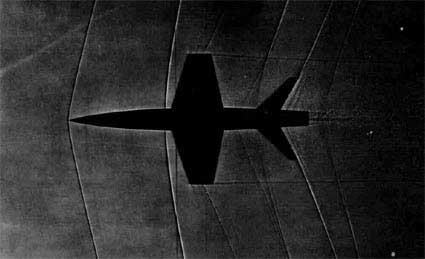
\includegraphics[width=0.3\textwidth]{img/ud-voln1.jpg}
    \caption{Модель самолета при обтекании сверхзвуковым потоком газа}
    \label{fig:plane}
\end{wrapfigure}
\textbf{Ударная волна} -- это распространяющийся по среде фронт резкого, почти мгновенного, изменения параметров среды: плотности, давления, температуры, скорости. Ударные волны называют также сильными разрывами или скачками. Причины возникновения ударных волн в газах – полеты со сверхзвуковыми скоростями (звуковой удар), истечения с большими скоростями через сопла, мощные взрывы, электрические разряды, интенсивное горение.
\\ \\Ударные волны на Рис. \ref{fig:plane} выглядят как темные линии: перед моделью (головная ударная волна), перед выступающими частями модели, за хвостом модели (хвостовой скачок).

\begin{wrapfigure}{l}{0.3\textwidth} %this figure will be at the right
    \centering
    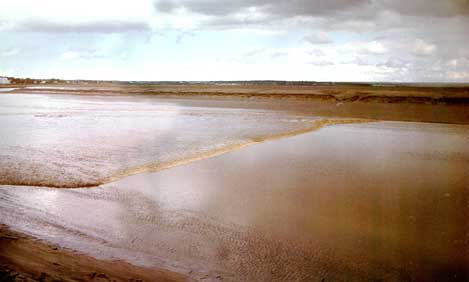
\includegraphics[width=0.3\textwidth]{img/bora.jpg}
    \caption{Бора на водной поверхности}
    \label{fig:bora}
\end{wrapfigure}
Ударные волны в воде носят название гидравлического удара. С этим явлением пришлось столкнуться при устройстве первых водопроводов: первоначально водопроводные задвижки перекрывали воду слишком быстро. Резкое прекращение тока воды вызывало ударную волну (гидравлический удар), распространявшуюся в трубе водопровода и часто вызывавшую разрыв такой трубы. Для решения этой проблемы в России был привлечен Жуковский, и она была успешно решена (1899). Ударные волны существуют и на поверхности воды: при открывании ворот шлюзов, при «запирании» течения реки (бора -- Рис. \ref{fig:bora}).

\begin{wrapfigure}{r}{0.25\textwidth} %this figure will be at the right
    \centering
    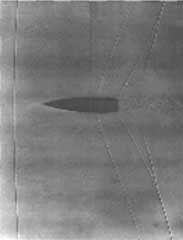
\includegraphics[width=0.3\textwidth]{img/bullet.jpg}
    \caption{Полет снаряда со сверхзвуковой скоростью}
    \label{fig:bullet}
\end{wrapfigure}
\noindent Ударные волны могут возникать и из первоначально непрерывных течений. Любая достаточно интенсивная волна сжатия порождает ударную волну из-за того, что в этих волнах задние частицы движутся быстрее впереди бегущих (нелинейное укручение фронта волны).
Ударные волны являются частью детонационных волн, волн конденсации (хорошо известным примером этого явления служат шлейфы тумана, остающиеся за самолетом при пролете через участки атмосферы с повышенной влажностью), могут возникать при взаимодействии лазерного излучения с веществом (светодетонационные волны). Сход снежной лавины также может рассматриваться как ударная волна.
В твердых телах ударные волны возникают при высокоскоростном соударении тел, в астрофизических условиях – при взрывах звезд.
Одним из примеров ударной волны является катастрофическое нарастание давки в охваченной паникой толпе, протискивающейся через узкий проход. Родственным явлением приходится затор в потоке транспорта. Ударные волны в газах были обнаружены в середине 19 в. в связи с развитием артиллерии, когда возросшая мощь артиллерийских орудий позволила метать снаряды со сверхзвуковой скоростью (Рис. \ref{fig:bullet}).
\\ \\ Введение понятия ударной волны приписывают немецкому ученому Бернхарду Риману (1876).
\\ \\ \textbf{Условия на фронте ударной волны}
\\ \\ При переходе через ударную волну должны выполняться общих законов сохранения массы, импульса и энергии. Соответствующие условия на поверхности волны – непрерывность потока вещества, потока импульса и потока энергии:
$$
\rho_{0} u_{0}=\rho u_{1}, 
$$
$$
p_{0}+\rho_{0} u_{0}^{2}=p_{1}+\rho_{1} u_{1}^{2},
$$
$$
h_{0}+\frac{u_{0}^{2}}{2}=h_{1}+\frac{u_{1}^{2}}{2}
$$
Здесь $r$ - плотность, $u$ - скорость, $p$ - давление, $h$ - теплосодержание газа. Индексом «0» отмечены параметры газа перед ударной волной, индексом «1» – за ней.\\ \\ Эти условия носят название \textbf{условий Ренкина-Гюгонио}, поскольку первыми из опубликованных работ, где были сформулированы эти условия, считаются работы британского инженера Вильяма Ренкина (1870) и французского баллистика Пьера Анри Гюгонио (1889).
\\ \\ Условия Ренкина – Гюгонио позволяют получить давление и плотность за фронтом ударной волны в зависимости от начальных данных (интенсивности ударной волны и давления и плотности перед ней):
$$
h_{0}-h_{1}+\frac{1}{2}\left(\frac{1}{\rho_{0}}+\frac{1}{\rho_{1}}\right)\left(p_{1}-p_{0}\right)=0
$$
Эта зависимость носит название адиабаты Гюгонио, или ударной адиабаты (Рис. \ref{fig:adia}).
\begin{figure}{0.3\textwidth} %this figure will be at the right
    \centering
    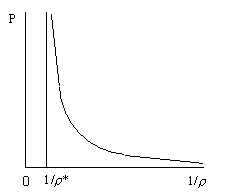
\includegraphics[width=0.3\textwidth]{img/adiabata.png}
    \caption{Адиабата Гюгонио}
    \label{fig:adia}
\end{figure}
Фиксируя на адиабате точку, соответствующую начальному состоянию перед ударной волной, получаем все возможные состояния за волной заданной интенсивности. Состояниям за скачками сжатия отвечают точки адиабаты, расположенные левее выбранной начальной точки, за скачками разрежения – правее. \\ \\Анализ адиабаты Гюгонио показывает, что давление, температура и скорость газа после прохождения скачка сжатия неограниченно возрастают при увеличении интенсивности скачка. В это же время плотность возрастает лишь в конечное число раз, сколь бы ни была велика интенсивность скачка. Количественно увеличение плотности зависит от молекулярных свойств среды, для воздуха максимальный рост 6 раз. При уменьшении амплитуды УВ она вырождается в слабый (звуковой) сигнал.


\end{document}
